\section{Hauptseite}\label{sec:main-page}

Die Hauptseite erreicht man, wenn man fulib.org das erste mal öffnet.
Dabei präsentiert sich der sogenannte Vier-Panel-Editor, welcher in Abbildung~\ref{fig:four-pane-editor}.

\begin{figure}
    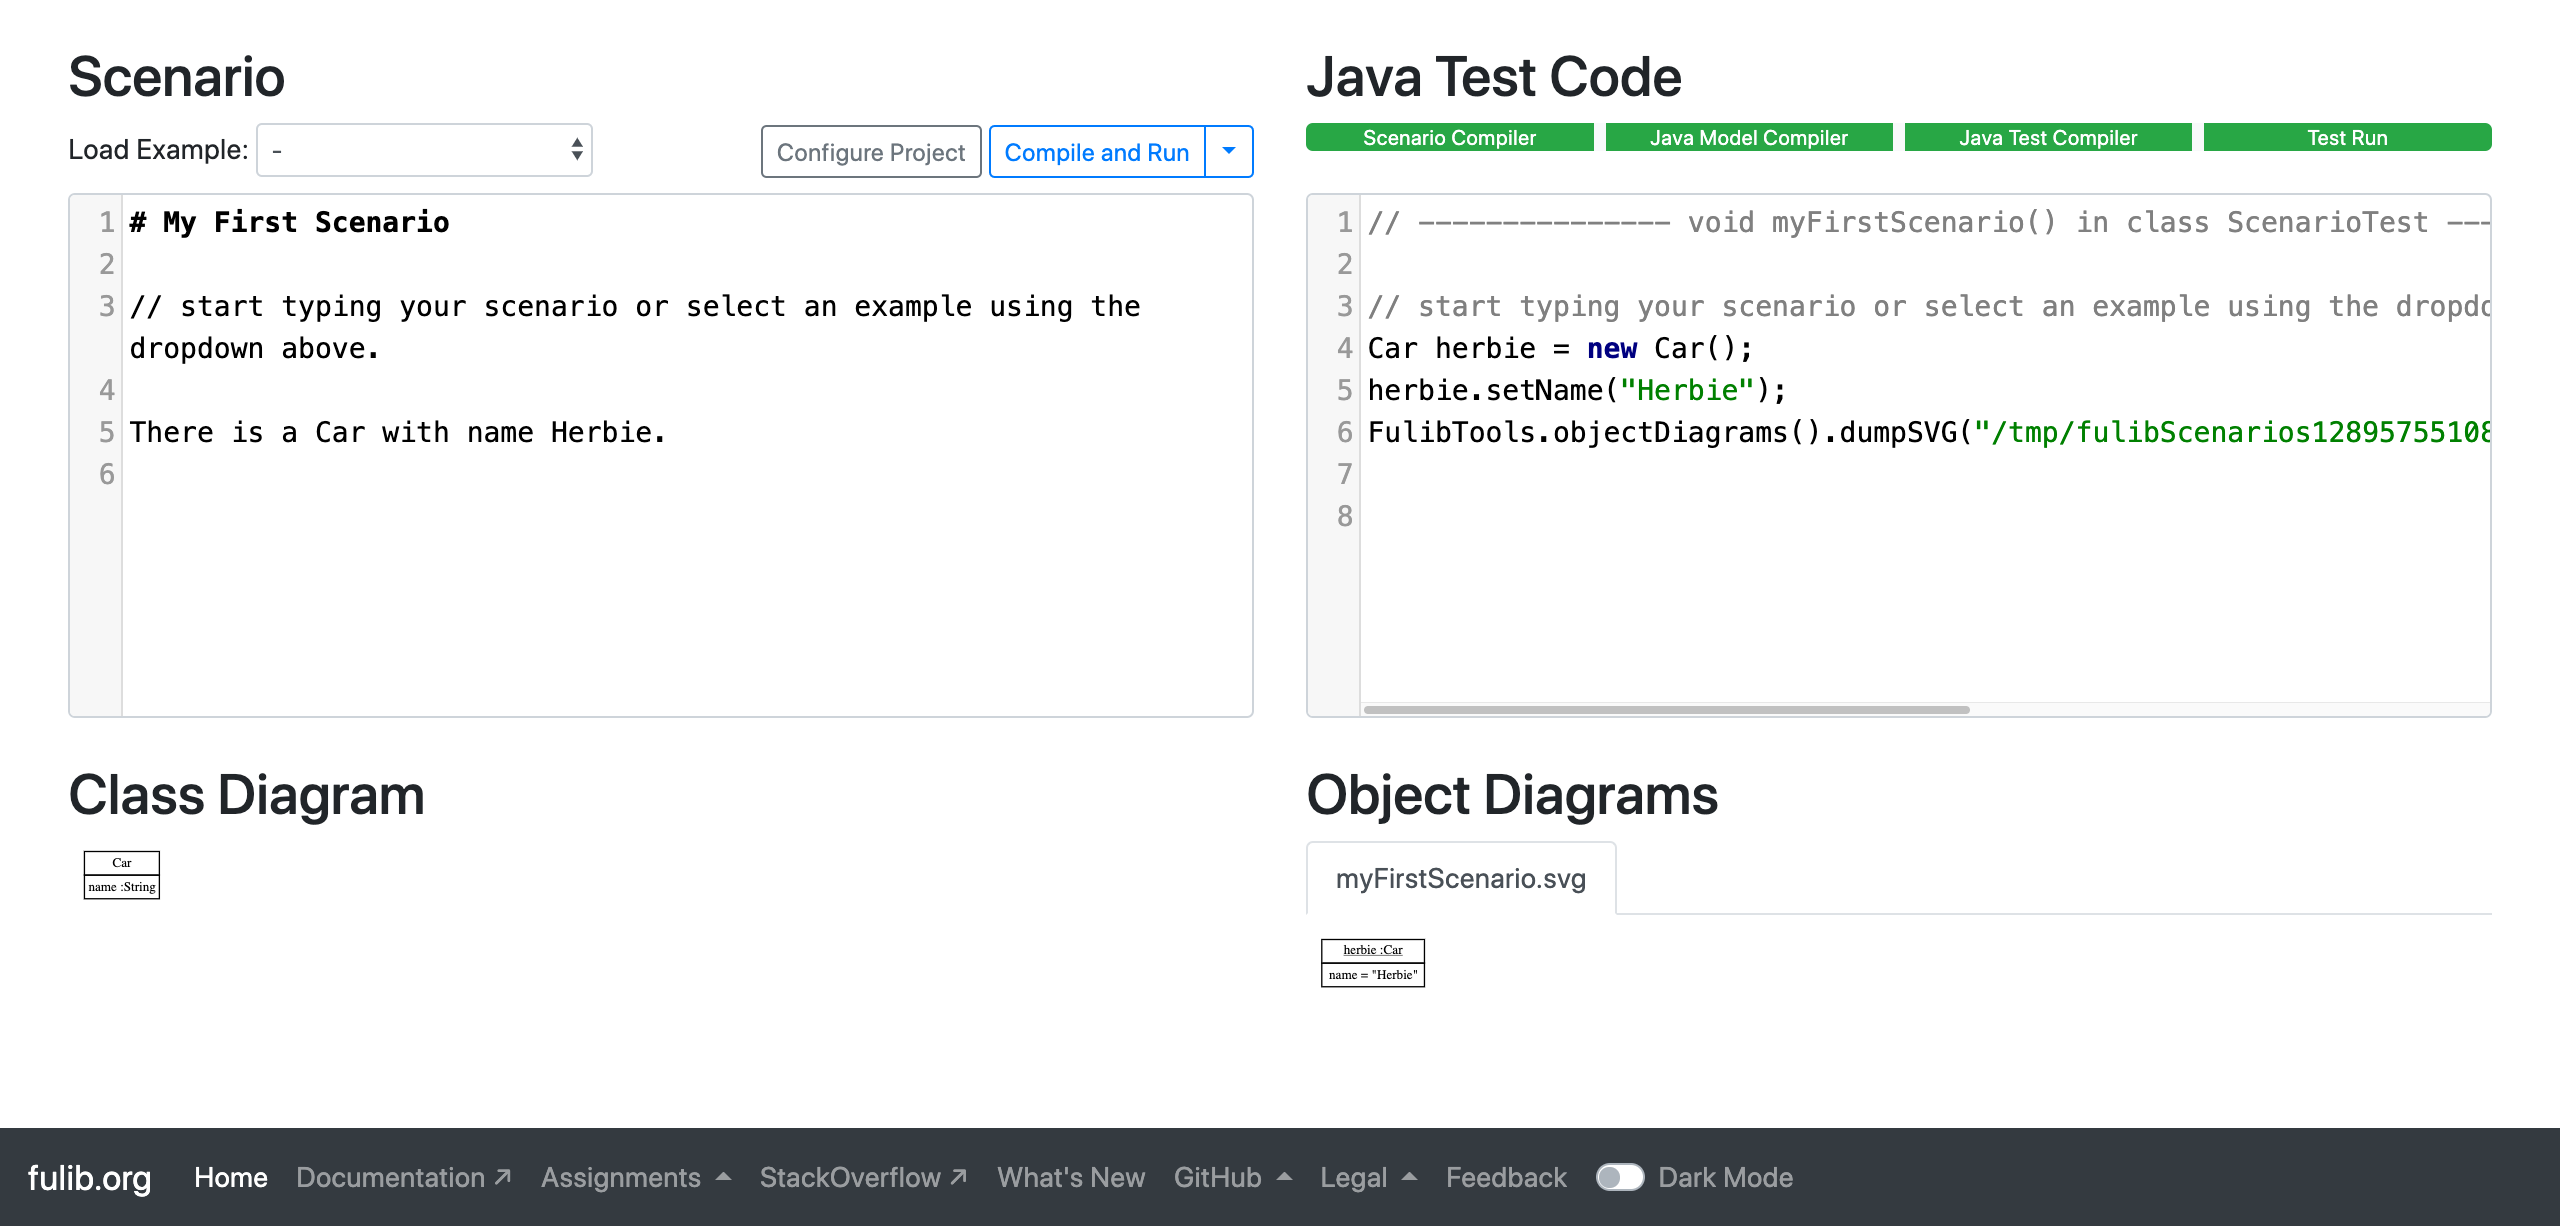
\includegraphics[width=\textwidth]{chapter/fulib.org/img/four-pane-editor.png}
    \caption{Der Vier-Panel-Editor auf der Hauptseite von fulib.org}
    \label{fig:four-pane-editor}
\end{figure}

Dieser zeigt oben links den Scenario-Editor sowie darüber dessen Toolbar.
Oben rechts gibt es ein Fenster für den generierten Java-Code, das auch die Konsolenausgabe des Compilers enthält.
Darüber zeigt eine Statusleiste, ob das Kompilieren und Ausführen erfolgreich war und wenn nicht, welches Tool fehlgeschlagen ist.
Im unteren Teil werden links das Klassendiagramm und rechts Objektdiagramme dargestellt.

Am unteren Rand der Seite befindet sich stets der Footer.
Dieser enthält Links zur Navigation innerhalb der Seite und zu externen Referenzen.
Außerdem finden sich darunter die Einstellungen für Datenschutz,
Möglichkeiten zum Hinterlassen von Feedback und zum Einsehen von Änderungen,
und die Schaltfläche zum Wechseln in den Nachtmodus.

\subsection{Interaktiver Spielplatz}\label{subsec:interactive-playground}

Die wichtigste Funktion der Hauptseite ist der Scenario-Editor.
Gibt man darin ein Scenario ein und klickt auf ``Compile and Run'' oder wartet einen Moment,
wird daraus Java-Code generiert und dessen Tests mit JUnit ausgeführt.
Das dabei entstehende Klassendiagramm sowie Objektdiagramme werden dann in den entsprechenden Bereichen angezeigt.
Um das sofortige Feedback zu erleichtern, wird das Scenario immer automatisch ausgeführt, wenn es länger als eine Sekunde unverändert blieb.
Somit muss man nicht manuell auf ``Compile and Run'' klicken.
Alternativ kann die automatische Ausführung im Dropdown neben dem ``Compile and Run''-Button deaktiviert werden.
Händisch lässt es sich dann immernoch durch Klick oder Verwenden der Testenkürzel auslösen.

Im Fenster für den Java-Code werden die Rümpfe sämtlicher Methoden angezeigt, die im Scenario verwendet wurden.
Davon ausgenommen sind aufgrund ihrer Trivialität Getter und Setter sowie diverse standardmäßig generierte Methoden.
Die Ausgabe des Scenario- und Java-Compilers sowie der JUnit-Testausführung werden ebenfalls in diesem Fenster angezeigt.
Dabei sind die Meldungen des Scenario-Compilers besonders relevant, da diese auf Fehler im Scenario hinweisen.

Objektdiagramme werden unter Tabs angeordnet.
Dies vermeidet Unübersichtlichkeit bei der Verwendung von vielen Diagram-Sätzen im Scenario.
Die einzelnen Darstellungen lassen sich dann getrennt voneinander betrachten.

\subsection{Tutorials}\label{subsec:tutorials}

Über dem Scenario-Editor befindet sich ein Auswahlfeld für vordefinierte Tutorials.
Wählt man eines davon aus, wird dessen Scenario-Text in den Editor übernommen und sofort ausgeführt.
Die Tutorials sind in Kategorien angeordnet und haben bauen in ihrer Reihenfolge aufeinander auf.
Somit werden die behandelten Sprachkonzepte zunehmend komplexer.

In den Tutorial-Scenarios ist beschreibender Text mit \code{//}-Kommentaren realisiert.
Diese bewirt, dass der Text auch im Java-Code auftaucht, was die Zuordnung vereinfacht.
Durch Abschnitte erfolgt eine visuelle Trennung von unabhängigen Teil-Scenarios.

Am Ende jedes Tutorials gibt es Links zu entsprechenden Abschnitten in der Dokumentation,
die detaillierte Informationen zu den verwendeten Sprachkonzepten enthalten.
Dazu gehören auch Grammatiken und häufige Problemfälle.

Die von Tutorials stammenden Scenarios können frei verändert werden.
Dadurch können die Sprachkonzepte direkt ausprobiert werden.
Lädt man das entsprechende Tutorial erneut, wird das vordefinierte Scenario verwendet und die Änderungen verworfen.

\subsection{Projektstarter}\label{subsec:project-starter}

\todo{
Gradle.
}

\subsection{Sicht der Studenten}\label{subsec:students-view}

\todo{
Feedback-Funktion.
Allgemeine Bewertung (PM).
Wünsche.
}

\subsection{Datensammlung}\label{subsec:data-collection}

\todo{
Request-Logging.
Fehleranalyse.
Lernverlauf.
Privacy-Einstellungen.
}
